\chapter{L'inversion de formes d'onde \label{fwi}}


L'inversion de formes d'onde (ou FWI, pour \emph{Full Waveform Inversion}) est une méthode quantitative d'imagerie développée dans un contexte géophysique. Elle permet de reconstruire des paramètres acoustiques ou élastiques par résolution d'un problème inverse, posé dans les années 80 par \cite{lailly} et \cite{tarantola_84}. Par opposition à des inversions du type tomographie des temps qui n'utilisent que partiellement les informations contenues dans les champs mesurés, l'inversion de formes d'onde utilise l'ensemble des données sans interprétation préalable des signaux enregistrés.\\

Le principe général est de calculer des données $\bm{d}_{cal}$ issues d'un modèle (résolution du problème direct)  puis de minimiser l'écart entre ces données et les données réelles $\bm{d}_{obs}$ issues de la mesure en modifiant les paramètres du modèle \citep{virieux_review}. Cette démarche est résumée en figure~\ref{schema_fwi}. \\


\begin{figure}[!h]
	\begin{tikzpicture}
		\node (init) [draw=black, align=center] at (0,0) {Paramètres initiaux \\ $\bm{m}_{0}$};
		\node (dir) [below=1cm of init , draw=black,align=center] {Problème direct :\\ éléments finis ou différences finies};
		\path[->, thick,shorten <=2pt,shorten >=2pt] (init) edge (dir);
		\node (fc) [draw=black,right=2cm of dir, align=center] {Fonction de coût \\ $C(\bm{m})=\frac{1}{2}||\bm{d}_{obs}-\bm{d}_{cal}(\bm{m})||^{2}$};
		\path[->, thick,shorten <=2pt,shorten >=2pt] (dir) edge (fc);
		\node (m) [draw=black, below right= and -5.5cm of dir, align=center] {Problème inverse : \\~\\ 
			\begin{minipage}{0.3\textwidth}
				\centering
				Calcul du gradient $C'(\bm{m})$
				Calcul du hessien $C''(\bm{m})$
			\end{minipage}
			\vline
			\begin{minipage}{0.23\textwidth}
				\centering
				~$\bm{\Delta m}=-(C'')^{-1}C'$
			\end{minipage}
			\vline
			\begin{minipage}{0.3\textwidth}
				\centering
				Mise à jour du modèle : \\ $\bm{m} := \bm{m}+ \bm{\Delta m}$
			\end{minipage}
		};
		\path[->, thick,shorten <=2pt,shorten >=2pt] (fc) edge (m);
		\path[->, thick,shorten <=2pt,shorten >=2pt] (m) edge (dir);		
	\end{tikzpicture} 
	\caption{ Schéma du principe de la FWI : le modèle courant est itérativement perturbé jusqu'à ce que le critère de convergence soit atteint.\label{schema_fwi}}
\end{figure}

L'ensemble des étapes de la FWI est détaillé par la suite. La résolution du problème direct est d'abord abordée, puis celle du problème inverse, avant d'évoquer quelques difficultés à prendre en compte lors de l'inversion. Un exemple d'application à des données sismiques est également présenté, ainsi que les spécificités de l'application de la FWI pour l'imagerie de soudure. \\

%"inversion approach resembles prestack, reverse-time mi-
%gration but differs in that the problem is formulated in
%terms of velocity (not reflectivity), and the method is
%fully iterative."PRATT99

%rodirguez 2014 : Full waveform
%inversion should not to be mistaken for migration techniques that
%are based on Claerbout’s ‘‘imaging principle’’ : J.F. Claerbout, Toward a unified theory of reflector mapping, Geophysics 36 (3)
%(1971) 467–481.which defines a
%reflectivity field by the ratio of upgoing and downgoing wave
%fields. Neverthelesss

\section{Problème direct \label{pd_dir}}

Dans le cas de l'imagerie par ultrasons, résoudre le problème direct revient à trouver la solution de l'équation d'onde linéarisée. Il est fréquent que l'hypothèse d'une propagation acoustique soit faite en prospection géophysique, notamment pour des acquisitions faites en mer. Cette approximation a pour but de réduire fortement le coût des calculs et est justifiée par le fait que la trace des ondes de compression soit dominante dans les données de mesures. De plus, en réduisant le nombre de paramètres du modèle, le problème est rendu moins non-linéaire. Cependant, cette approximation ne permet pas une caractérisation complète du milieu. Pour une application en CND, elle demande un pré-traitement parcimonieux des données et retire notamment la précision potentielle qu'offrent les ondes de cisaillement par leur faible longueur d'onde.\\~\\




 Pour résoudre l'équation d'onde, parmi les approches qui nécessitent de faire le moins d'hypothèse sur le champ d'onde et sur le milieu de propagation figurent les différences finies et les éléments finis. Les différences finies sont les plus faciles à développer et à implémenter. Elles permettent de discrétiser les dérivées temporelles et spatiales par des différences d'ordre 2 \citep{virieux_86} ou d'ordre 4 \citep{levander}. Cependant, contrairement aux éléments finis, elles imposent, en général, l'utilisation de grilles régulières et ne permettent donc pas d'adapter localement le pas de grille à la géométrie ou à la complexité du milieu. \\ Les éléments finis se prêtent mieux à une description du milieu par un maillage non-structuré. Leur solution est développée sur des bases de fonction (d'ordre élevé pour les éléments finis spectraux) et permettent de prendre simplement en compte les conditions limites.\\
 
Deux types de conditions limites sont nécessaires pour le modèle de soudure à 2 dimensions (2D) : une condition parfaitement réfléchissante (condition de Dirichlet) au niveau des surfaces de la plaque (en considérant une mesure dans l'air, le couplage fluide structure est négligeable) et une condition absorbante pour représenter la plaque loin de la zone d'étude (cf figure~\ref{BC}). Les conditions absorbantes sont modélisées à l'aide de zones éponges \emph{Perfectly Matched Layers} (PML,\cite{berenger}) qui simulent une forte atténuation dans cette zone de manière anisotrope (seule la composante normale de l'onde est atténuée, ce qui les rend imparfaites).\\

\begin{figure}[!h]
	\centering
	\begin{tikzpicture}
		\node at(5,-1) {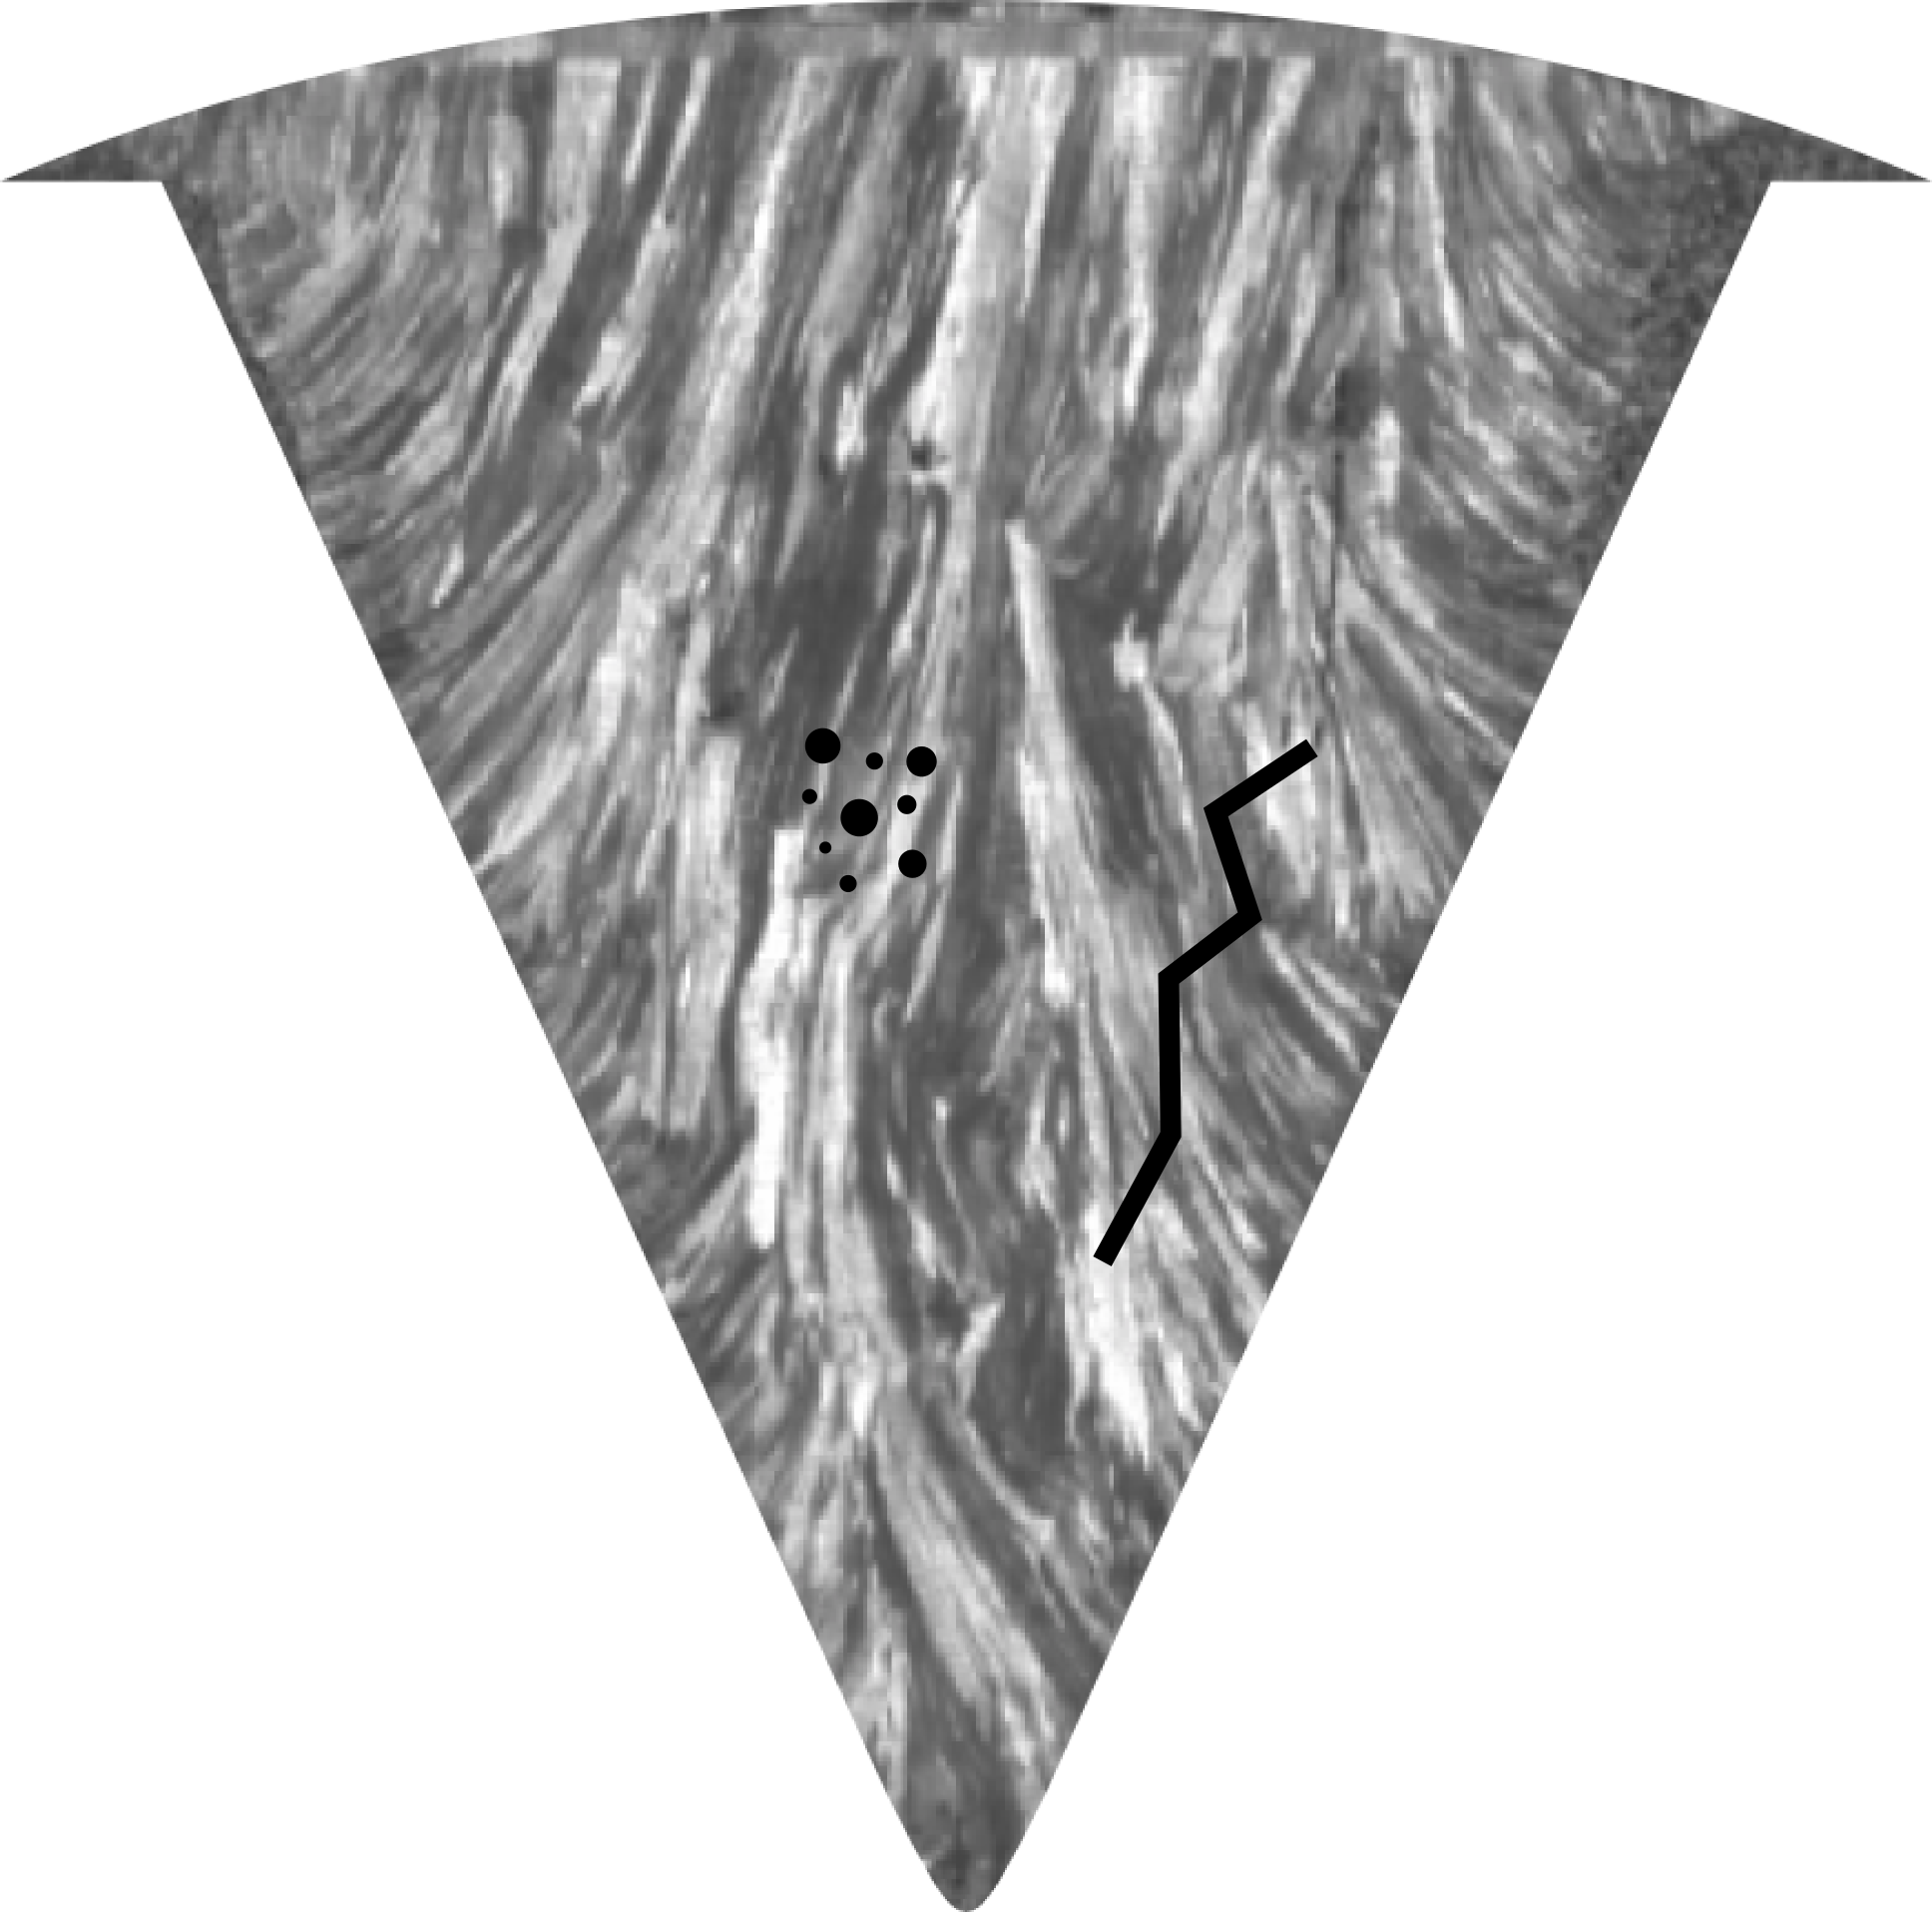
\includegraphics[scale=0.0365]{img/anisotrope2.png}};
		\draw (0,0) -- (9,0) ;
		\draw (0,-2) -- (9,-2) ;
		%\filldraw [fill=gray, fill opacity=0.5, draw=none] (3.5,0) -- (4.5,-2) -- (5.5,0)  ;
		\node (centre) at (5,-1) {};
		\node (soudure) at (7,-2.5) {soudure};
		\draw[<-,thick] (centre) -- (soudure);
		\node (fs) [align=left] at (1.8,0.3) {Condition de Dirichlet}	;
		\node (fs2)[align=left] at (1.8,-2.3) {Condition de Dirichlet};
		\draw[dotted] (0,0) -- (0,-2);
		\draw[dotted] (9,0) -- (9,-2);
		\node (g) [align=center] at (-1.3,-1) {Conditions \\ absorbantes \\ (PML)};
		\node (d) [align=center] at (10.3	,-1	) {Conditions \\ absorbantes \\ (PML)};
		\draw[dashed] (0,0) -- (-1,0);
		\draw[dashed] (0,-2) -- (-1,-2);
		\draw[dashed] (9,0) -- (10,0);
		\draw[dashed] (9,-2) -- (10,-2);
		\node (x) at (-3,0) {$\bm{e}_{x}$};
		\draw[<-,thick] (x)-- +(-1,0);
		\node (z) at (-4,-1)  {$\bm{e}_{z}$};
		\draw[<-,thick] (z)--+(0,1);
		\node (z) at (-5,0)  {$\bm{e}_{y}$};
		\draw[thick] (z)+(0.5,0) circle [radius=0.1];
		\draw (z)+(0.5,0) node[cross=2.2pt,rotate=0,black] {};
	\end{tikzpicture}
	\caption{Représentation des deux types de conditions limites du modèle de soudure 2D.\label{BC}}
\end{figure}


Le problème peut être résolu dans le domaine temporel ou dans le domaine fréquentiel \citep{vigh_2008}. Le domaine temporel facilite la sélection des arrivées d'ondes par fenêtrage temporel mais présente une plus forte sensibilité au phénomène de saut de phase (décrit dans le paragraphe~\ref{fwi:choix_modele}).  De plus, la résolution par méthodes numériques dans le domaine temporel impose un critère de stabilité Courant-Friedrichs-Lewy (CFL) qui peut être contraignant, surtout en 3D. Dans le domaine fréquentiel, l'équation d'onde construit la solution stationnaire, ce qui revient à résoudre un système d'équations linéaires. Il est alors possible d'utiliser des méthodes de résolution directe du type décomposition LU, bien qu'elles demandent beaucoup de mémoire, notamment pour des problèmes comportant un grand nombre d'inconnues.  Les principaux avantages d'une résolution du problème direct dans le domaine fréquentiel sont donc d'intégrer facilement les phénomènes d'atténuation et de permettre une sélection fine des fréquences d'intérêt. 







\section{Problème inverse}

Le problème inverse considéré est un problème d'optimisation locale visant à réduire l'écart entre les données observées $\bm{d}_{obs}$ et les données calculées $\bm{d}_{cal}(\bm{m})$ pour chaque couple source-récepteur, en ajustant le modèle constitué de M paramètres $\bm{m}$. L'idée est donc de minimiser la norme au sens des moindres carrés de la différence $\bm{d}_{obs}-\bm{d}_{cal}(\bm{m})$ sur l'ensemble des couples source-récepteurs définie par la relation : 
\begin{equation}
	C(\bm{m})=\frac{1}{2}||\bm{d}_{obs}-\bm{d}_{cal}(\bm{m})||^{2}\text{.}
	\label{norm}
\end{equation}
 Le minimum de cette fonction de coût est atteint lorsque la dérivée par rapport aux paramètres du modèle s'annule. Un développement de Taylor au second ordre de $C(\bm{m}+ \bm{\Delta m})$ permet d'écrire : 
 \begin{equation}
 	\frac{\dd C(\bm{m}+\bm{\Delta m})}{\dd m_{i}}= \frac{\dd C(\bm{m})}{\dd m_{i}} + \displaystyle\sum_{j}^{M} \frac{\dd^{2} C(\bm{m})}{\dd m_{j} \dd m_{i}}\Delta m_{j}\text{.}
 	\label{fwi:taylor}
 \end{equation}
Les termes d'ordres plus élevés du problème inverse sont nuls si le problème direct est linéaire. Le minimum de la fonction de coût est alors atteint en une seule itération en annulant la dérivée : 
\begin{equation}
	\frac{\dd C(\bm{m}+\bm{\Delta m})}{\dd m_{i}} = 0 ~~~~~\Leftrightarrow ~~~~~ \Delta m _{j} = -\left( \frac{\dd ^{2} C(\bm{m})}{\dd m_{j} \dd m_{i} }\right)^{-1} \frac{\dd C (\bm{m})}{\dd m_{i}} \text{.}
\end{equation}
En FWI, le problème direct est non-linéaire et le problème inverse est linéarisé : les termes d'ordres supérieurs de la série~\ref{fwi:taylor} sont négligés et l'inversion est réalisée sur plusieurs itérations.\\
La perturbation du modèle courant à l'itération considérée est alors définie par la direction de descente donnée par le gradient et par la courbure de la fonction de coût donnée par la dérivée du gradient (le hessien).



\subsection{Calcul du gradient}

D'après l'expression de la norme~\ref{norm}, sa dérivée par rapport aux paramètres $\bm{m}$ (le gradient) est : 
\begin{equation}
	 G_{i}(\bm{m})=\frac{\dd C (\bm{m})}{\dd m_{i}} = -\tr{\left( \frac{\dd \bm{d}_{cal}(\bm{m}) }{\dd m_{i}} \right)} ( \bm{d}_{obs} - \bm{d}_{cal}(\bm{m})) \text{.}
	 \label{eq_grad}
\end{equation}\\



Dans le domaine temporel, le problème direct décrit au paragraphe précédent~(\ref{pd_dir}) peut se mettre sous la forme :
\begin{equation}
	\bm{A}(\bm{m},\bm{x},t)\bm{d}_{cal}(\bm{m},\bm{x},t)=\bm{s}(\bm{x},t)\text{,}
	\label{eq_pb_dir}
\end{equation}
où $\bm{x}$ est la variable d'espace. $\bm{A}$ est un opérateur correspondant à l'équation d'onde et $\bm{s}$ est le terme source. On note $\bm{\tilde{d}}_{cal}$ et $\bm{\tilde{d}}_{obs}$ les vecteurs des données étendus de façon à passer leur dimension du nombre de récepteur à celle de l'espace du problème direct. La dérivée de l'équation~\ref{eq_pb_dir} par rapport à $\bm{m}$ s'écrit : 
\begin{equation}
	\bm{A} \frac{\dd \bm{\tilde{d}}_{cal}(\bm{m})}{\dd m_{i}} + \frac{\dd \bm{A}}{\dd m_{i}}\bm{\tilde{d}}_{cal}(\bm{m}) = \bm{0} \text{.}
\end{equation}

On a donc : 
\begin{equation}
	\tr{\left( \frac{\dd \bm{\tilde{d}}_{cal}(\bm{m})}{\dd \bm{m}}  \right)} = - \tr{\bm{\tilde{d}}_{cal}(\bm{m})} \tr{\left( \frac{\dd \bm{A}}{\dd \bm{m}} \right)} \tr{\bm{A}^{-1}}.
	\label{sub}
\end{equation} 	

Finalement, en reportant cette expression dans l'équation~\ref{eq_grad}, on obtient l'expression du gradient  
\begin{equation}
	 \frac{\dd C (\bm{m})}{\dd m_{i}} = \tr{\bm{\tilde{d}}_{cal}(\bm{m})}  \tr{\left( \frac{\dd \bm{A}}{\dd m_{i}}\right)} \tr{\bm{A}^{-1}} (\bm{\tilde{d}}_{obs} - \bm{\tilde{d}}_{cal}(\bm{m})) = \tr{\bm{\tilde{d}}_{cal}(\bm{m})} \tr{\left( \frac{\dd \bm{A}}{\dd m_{i}}\right)} \bm{\lambda}.
	 \label{fwi:eq_grad2}
\end{equation}


Le champ $\bm{\lambda}$ correspond donc à la rétropopagation des résidus $( \bm{\tilde{d}}_{obs} - \bm{\tilde{d}}_{cal}(\bm{m}))$ qui, de manière comparable au retournement temporel \citep{prada_2002}, permet une focalisation sur les éléments diffractant absents du modèle initial. Cette expression du gradient peut également être obtenu par le formalise de l'état adjoint \citep{plessix}.\\
Finalement, le gradient découle donc du calcul de deux problèmes directs : 
\begin{equation*}
	\bm{A}(\bm{m})\bm{\tilde{d}}_{cal}(\bm{m})=\bm{s} ~~~~~~~\text{et}~~~~~~~\bm{A}(\bm{m})\bm{\lambda} (\bm{m})=( \bm{\tilde{d}}_{obs} - \bm{\tilde{d}}_{cal}(\bm{m})),
\end{equation*}
en notant que $\tr{\bm{A}}=\bm{A}$ par réciprocité spatiale du problème direct.\\


La substitution~\ref{sub} permet d'éviter le calcul de la matrice de sensibilité $\tr{\left( \frac{\dd \bm{\tilde{d}}_{cal}(\bm{m}) }{\dd m_{i}} \right)}$, menant au calcul plus léger de $\frac{\dd \bm{A}}{\dd m_{i}}$ qui est très creux et dont on connaît les solutions analytiques. Ce dernier terme agit comme une pondération du champ $\bm{\lambda}$ liée au diagramme de rayonnement pour chaque paramètre.


\subsection{Estimation du hessien}

Dans nos applications, la méthode d'optimisation choisie pour la FWI est une méthode quasi-Newton qui propose d'utiliser une version approximée de l'inverse du hessien, estimée à partir de valeurs précédentes du gradient, évitant ainsi le calcul du hessien. \cite{brossier_2009} montrent que cette méthode, développée avec l'algorithme L-BFGS, est plus performante que la méthode du gradient conjugué préconditionné en terme de convergence. 


\subsection{Régularisation}

Le problème étant mal-posé, il est nécessaire de limiter les artefacts haute fréquence venant perturber l'estimation $\bm{\Delta m}$. Pour cela, il est possible d'ajouter un terme de pondération à la fonction de coût qui permet de lisser le modèle. Ce lissage peut aussi être directement appliqué à $\bm{\Delta m}$ sous forme de filtre spatial adapté à la longueur d'onde correspondant à la fréquence d'inversion. Cette seconde stratégie est utilisée par la suite.

\section{Problématiques liées à l'inversion}

\subsection{Choix du modèle initial \label{fwi:choix_modele}}
Afin d'assurer une convergence vers le minimum global, il est nécessaire que le modèle initial se situe dans le bassin d'attraction de la fonctionnelle à réduire. Pour cela, il faut s'assurer que le modèle soit cinématiquement acceptable en levant l’ambiguïté sur la phase. Les données temporelles issues de ce modèle doivent donc avoir un décalage de moins d'une demi-période par rapport aux données observées vraies. Si cette condition n'est pas respectée, l'algorithme ne permettra pas un bon réajustement des phases et convergera vers un minimum local, comme l'illustre la figure~\ref{ambig_phase}.%\todo{application numérique : \% de retard ?}

\begin{figure}[!h]
	\centering
	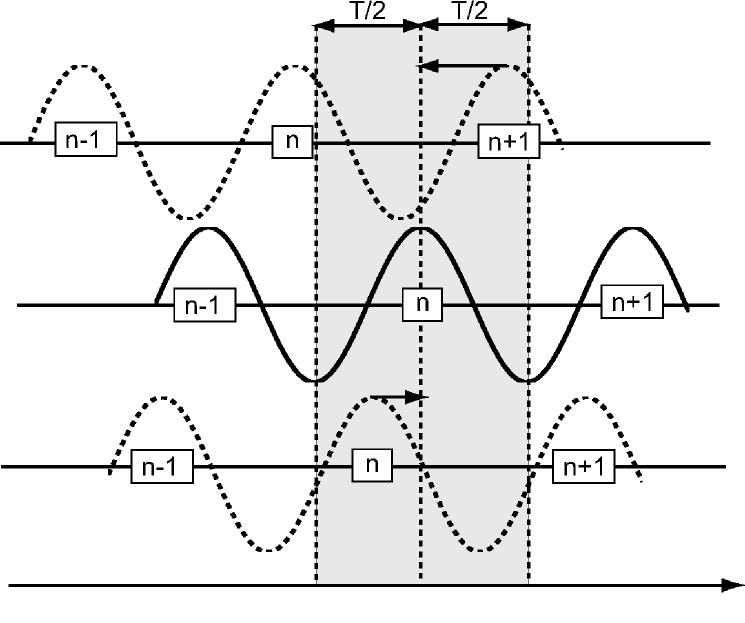
\includegraphics[height=6cm]{img/ambig_phase.png}
	\caption{Illustration de l'ambiguïté sur la phase (extraite de \cite{brossier_these}). En haut, le déphasage est supérieur à $T/2$, les arches sont mal ajustées par rapport à la donnée vrai du milieu. En bas, le déphasage est inférieur à $T/2$, les phases sont bien ajustées. \label{ambig_phase}}
\end{figure}

À défaut de disposer d'un modèle initial cinématiquement acceptable, il est possible d'appliquer un ensemble de stratégies permettant de limiter ces artefacts : introduire progressivement les sources ou récepteurs les plus éloignés, rallonger progressivement les temps d'acquisition, et inverser prioritairement les données basses fréquences. Ces stratégies sont essentielles pour une bonne convergence vers le modèle vrai inconnu.


En sismologie, une image issue de tomographie des temps peut fournir un modèle initial assez précis. Dans cette étude, on considère que peu d'informations sont connues sur les paramètres élastiques de la soudure et le modèle initial choisi est uniforme, bien qu'il serait intéressant d'établir un modèle initial de soudure caractéristique (cf chapitre~\ref{applications}).


\subsection{Choix de la paramétrisation et inversion multi-paramètres}
L'inversion multi-paramètres implique plus de degrés de liberté dans le problème et rend donc l'inversion plus difficile, en raison des possibles ambiguïtés sur les effets des paramètres sur les données. Ainsi, ces paramètres peuvent avoir des effets, couplés ou non, de différentes natures (cinématiques ou dynamiques) et de différentes amplitudes sur les données. Il faut donc choisir les paramètres à inverser de manière à ce qu'ils décrivent au mieux (de manière complémentaire si possible) les propriétés du milieu à imager. Par exemple, les paramètres de vitesse influencent le champ en terme de temps de vol, tandis que la densité ou l'impédance jouent davantage sur l'amplitude du champ réfléchi.\\


À chaque ensemble de paramètres est associé localement un diagramme de rayonnement lié à l'expression de leur différentielle~\citep{forgues} : c'est l'approximation du simple diffraction à la base de la linéarisation du problème inverse. Ces diagrammes traduisent la capacité de chaque paramètre à décrire le rayonnement d'une onde plane sur un point diffractant, en fonction de l'angle de diffraction. Quelques exemples de diagrammes de rayonnement sont présentés en figure~\ref{rayonnement}, où $\kappa$ est le module d'incompressibilité, $\rho$ est la densité, $v_{p}$ est la vitesse des ondes longitudinales se propageant suivant $z$ et $I_{p}$ est l'impédance, tels que : 
\begin{equation*}
	I_{p}=\sqrt{\kappa \rho}~~~~~\text{et}~~~~~\kappa=\rho v_{p}\text{.}
\end{equation*}
Ces diagrammes correspondent au rayonnement des paramètres acoustiques dans un milieu isotrope. En milieu anisotrope, ces diagrammes sont plus difficiles à estimer analytiquement et nécessite une bonne connaissance de l'anisotropie du milieu.\\

Ajouté à l'illumination restreinte  par le système d'acquisition, ce rayonnement peut filtrer le spectre en nombre d'onde du milieu reconstitué. 


\begin{figure}[!h]
	%\centering
	\hspace{-1cm}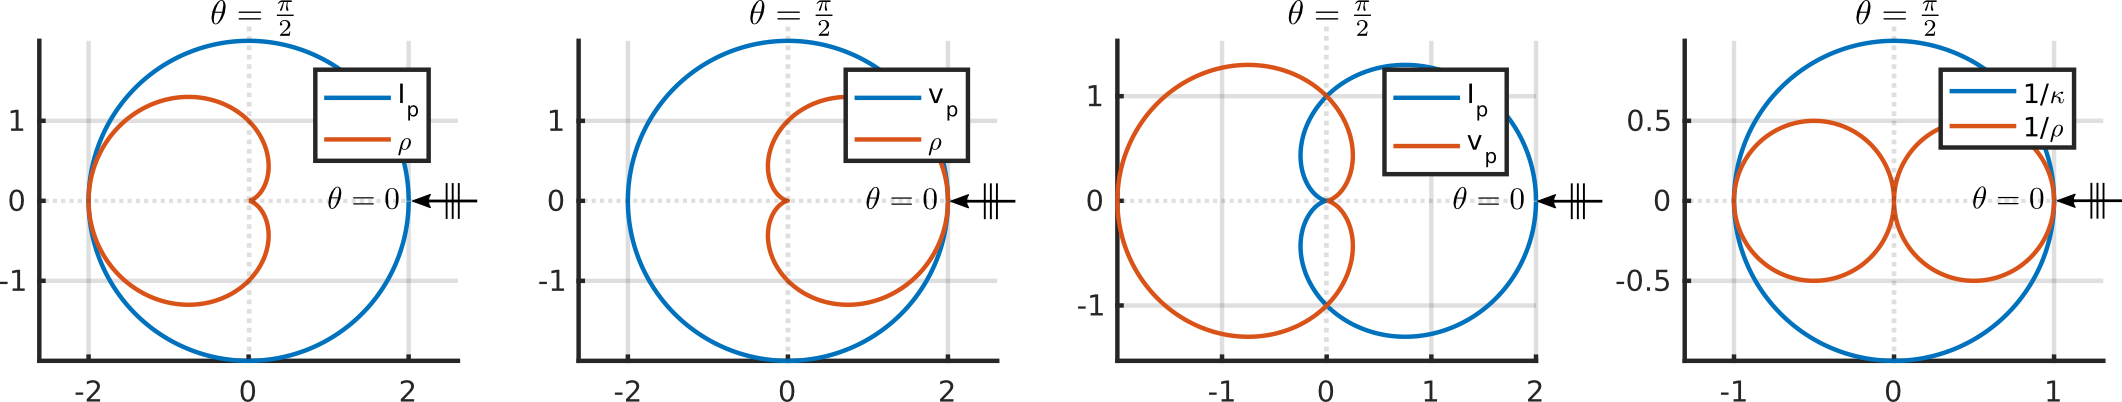
\includegraphics[width=1.1\textwidth]{img/rayonnement.png}
	\caption{Diagrammes de rayonnement pour différentes paramétrisations d'un milieu acoustique (amplitudes relatives) tracés d'après \cite{forgues}. Pour une onde incidente en $\theta=0$, l'amplitude de l'onde rayonnée localement dans une direction $\theta$ sera décrite différemment en fonction de la paramétrisation du problème. \label{rayonnement}}
\end{figure}
%forgues : p.156

\subsection{Estimation de la source}
Pour que les données calculées puissent être comparées aux données observées, il est nécessaire que les termes sources à l'origine des deux champs soit semblables. Ce terme source est linéairement lié au champ (cf équation~\ref{eq_pb_dir}) et il peut donc être calculé par la résolution d'un problème linéaire \citep{pratt_99} dont la solution est, dans le domaine fréquentiel, donnée par 
\begin{equation}
s=\frac{\tr{\bm{d}_{cal}(\bm{m})^{*}}\bm{d}_{obs}^{*}}{\bm{d}_{cal}(\tr{\bm{m})^{*}}\bm{d}_{cal}(\bm{m})^{*}}\text{.}
\end{equation}
où $^{*}$ est l'opérateur conjugué.
 


\section{Exemple d'application en géophysique}

Dans cette section, on se propose de présenter un exemple d'application de la FWI à des données sismologiques dans le cadre de la prospection pétrolière, réalisés par \cite{sirgue_valhall}. Dans ce domaine, les mesures étant rares et coûteuses, l'exploitation des données doit être efficace en terme de qualité d'image. C'est pourquoi une méthode comme la FWI y est adaptée, bien qu'elle nécessite beaucoup de ressources informatiques.\\

L'exemple choisi est issu d'une acquisition en fond de mer du Nord (\emph{Ocean Bottom Cable}) par hydrophones, au niveau de Valhall en Norvège. Ce dispositif est constitué de 120 km de câbles équipés de 2414 récepteurs, espacés de 50 m, couvrant 45 km$^{2}$ (cf figure~\ref{dispositif_valhall}). 50000 points sources sont excités par canon à air.

\begin{figure}[!h]
	\centering
	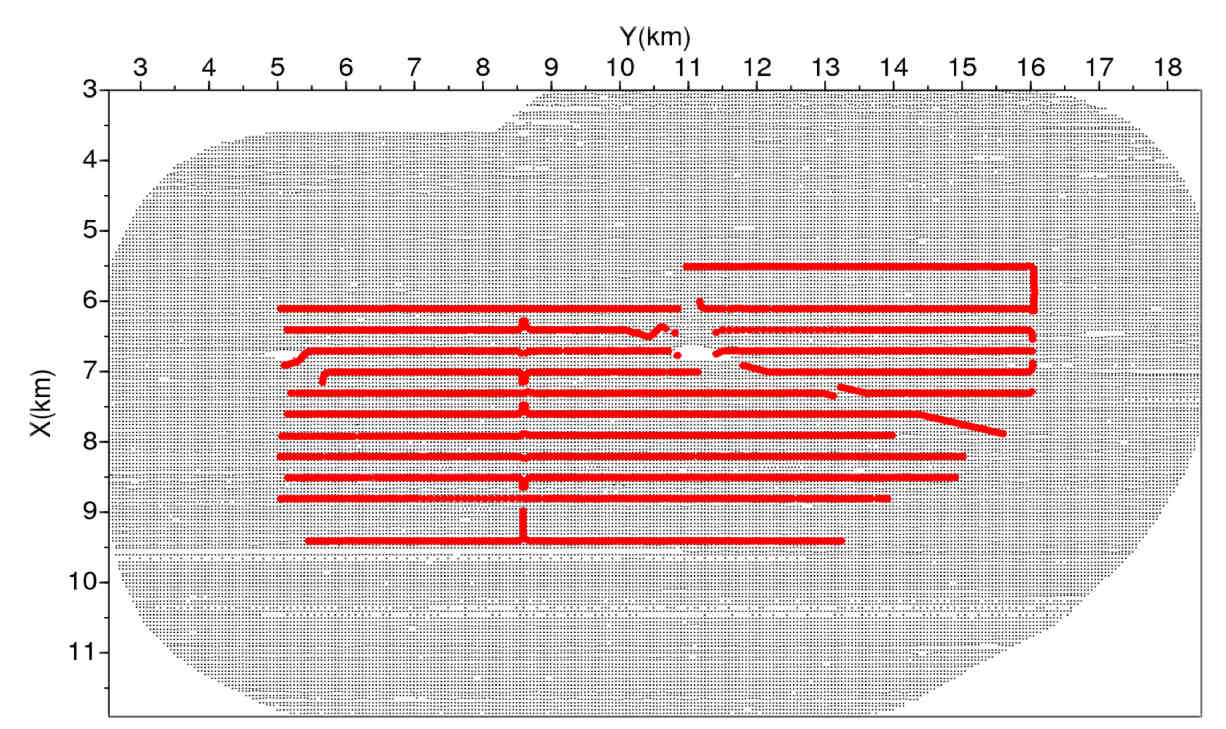
\includegraphics[height=5cm]{img/dispo_valhall.jpg}
	\caption{Schéma du dispositif d'acquisition pour les mesure sur Valhall. L'antenne de récepteur est représenté en rouge (l'espacement entre les câble est d'environ 300 m) et les positions des sources sont données par les points gris (image extraite de \cite{sirgue_valhall}).\label{dispositif_valhall} }
\end{figure}

Le résultat du post-traitement des données est présenté en figure~\ref{valhall}. Cette figure confronte les images obtenues par une méthode d'imagerie conventionnelle (tomographie des temps en réflexion) et celles obtenues par FWI de 3.5 à 7 Hz, avec pour modèle initial la carte de vitesse donnée par tomographie.

\begin{figure}[!h]
    \centering
    \begin{subfigure}[b]{0.4\textwidth}
        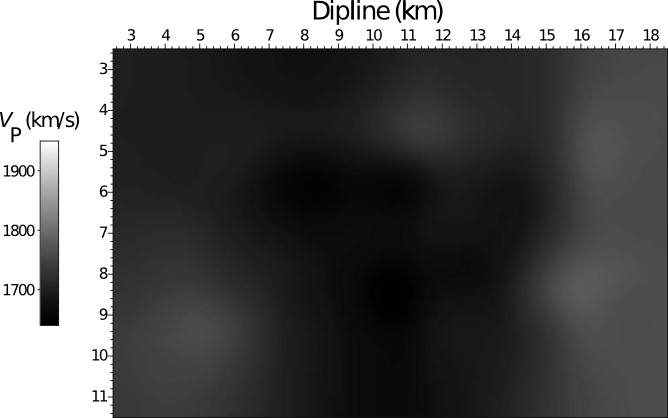
\includegraphics[width=\textwidth]{img/geophy1.png}
        \caption{ Par tomographie des temps en réflexion. Coupe à 150 m de profondeur.}
        \label{}
    \end{subfigure}
    \hspace{0.5cm}
    \begin{subfigure}[b]{0.4\textwidth}
        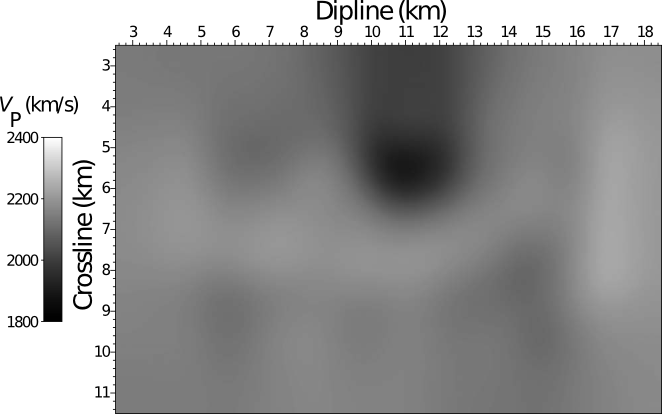
\includegraphics[width=\textwidth]{img/geophy2.png}
        \caption{Par tomographie des temps en réflexion. Coupe à 1050 m de profondeur.}
        \label{}
    \end{subfigure}\\[0.5cm]
    \begin{subfigure}[b]{0.4\textwidth}
        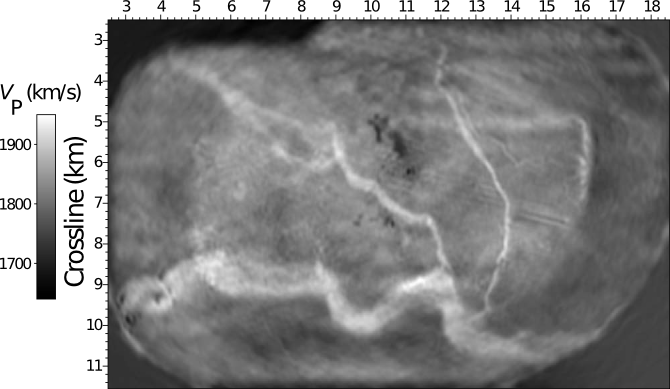
\includegraphics[width=\textwidth]{img/geophy3.png}
        \caption{Par FWI. Coupe à 150 m de profondeur.}
        \label{}
    \end{subfigure}
    \hspace{0.5cm}
    \begin{subfigure}[b]{0.4\textwidth}
        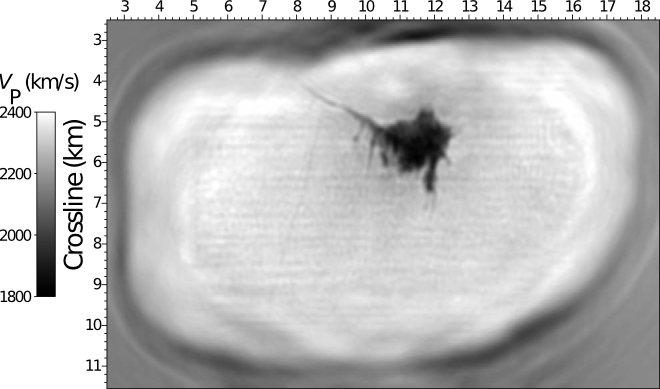
\includegraphics[width=\textwidth]{img/geophy4.png}
        \caption{Par FWI. Coupe à 1050 m de profondeur.}
        \label{}
    \end{subfigure}
    \caption{Images des vitesses dans le champ de Valhall (extraites de \cite{sirgue_valhall}).\label{valhall}}
\end{figure} 
   
La FWI permet de faire apparaître des empreintes sédimentaires d'un réseau paléo-fluvial à 150 m de profondeur, invisible sur la tomographie. À 1050 m, les contours du nuage de gaz (en noir) situé au-dessus du réservoir proprement dit sont également mieux défini par la FWI. Cette méthode d'imagerie peut donc constituer une aide précieuse pour l'analyse des sous-sols et pour la mise en place des stratégies de forage au cours de l'exploitation du réservoir (sur 10 à 50 ans).\\

On comprend par la qualité d'image qu'offre la FWI qu'il est intéressant de varier ses applications. On peut citer l'utilisation des ondes électromagnétiques (données radar, par exemple ~\cite{lopes}) ou encore l'imagerie médicale. Dans ce domaine, \cite{oberai_03,oberai_04} reconstruisent le module d'élasticité en équilibre statique d'une imitation de tissu humain.\\

En comparaison avec l'imagerie terrestre, l'application de la FWI à l'imagerie par ultrasons impose un changement d'échelle, dont le rapport est $10^5$. Elle impose aussi de prendre en compte les spécificités du dispositif d'acquisition, ainsi que celles des propriétés géométriques et élastiques du milieu à imager.







%
%-guide d'onde
%-acquisition en surface seulement, et problématique de la soudure bombée
%-anisotropie (cf image soudure) forte, qui touche not. les ondes S.
%-acquisition horizontale pas idéale pour inverser la vitesse horizontale (car petits offsets et peu de courbure de rayon comme en géophys) (discuter le choix des paramètres à inverser compte-tenu de la configuration)
%-sources et récepteurs mobiles 
%-geophysique, dispositif de surface, donc on ne considère que les diffractions rayonnant vers la surface (soit angle de diffraction de max 180°)(Forgues, pages 160). En CND, on illumine des deux côté


%\begin{figure}
%	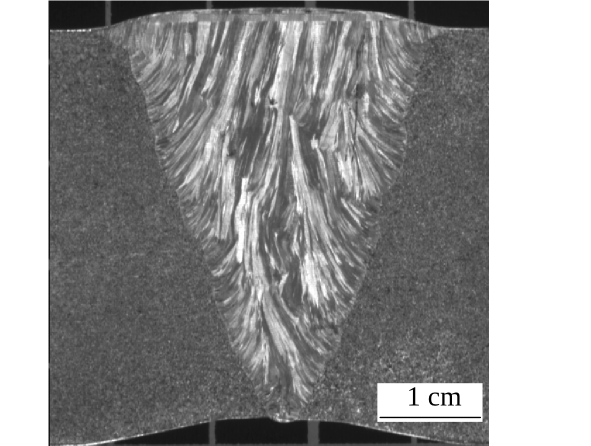
\includegraphics[height=5cm]{./img/soudure1.png}
%	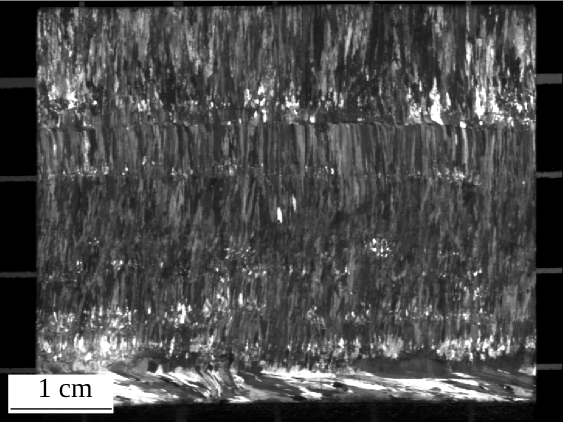
\includegraphics[height=5cm]{./img/soudure2.png}
%	\caption{Macrographie d'une soudure industrielle en acier inoxydable en acier austénitique \citep{chassignole}. À gauche : coupe dans le plan $(x,z)$, à droite : coupe dans le plan $(x,y)$.}
%\end{figure}

%grains colonnaires

%p91 potel bruneau : données "d'aspect limité" : il n'es tpas possible de tourner autour de l'obstace. On colpense la perte d'info en réalisant les mesures sur plusieurs freq et possibilité de déplacer capteur.




%\subsection{sensibilité au bruit ?}
%
%\todo[inline]{Les impasses volontairement faites : \\
%	- détail de la discrétisation différences finies / détail des calculs FEM\\	
%}
%
%
%\todo[inline]{born approx}
